\documentclass{beamer}
\usepackage[utf8]{inputenc}
\usepackage[T1]{fontenc}
\title{Ruang Topologi}
\subtitle{\textit{Closed Sets, Closures. Interior of Sets}}
\date[]{2024/2025}
\author[Fritz]{Fritz Adelbertus Sitindaon}

% \usetheme{fritz}
% ===== Setup Font =====
\usepackage[sfdefault,lf]{carlito}
\usepackage[T1]{fontenc}
\renewcommand*\oldstylenums[1]{\carlitoOsF #1}

% ==== Import Math Packages =====
\usepackage{amsmath, amssymb, amsthm}
\usepackage{mathtools}

\def\R{\mathbb{R}}
\def\P{\mathbb{P}}
\def\N{\mathbb{N}}

\begin{document}

\begin{frame}
\titlepage
\end{frame}

\begin{frame}{Outline}
    \tableofcontents
\end{frame}

\section{Review}

\begin{frame}{Materi Sebelumnya}
    \begin{tcolorbox}[enhanced,title=Usual Topology, frame style tile={width=\paperwidth}{\wallpaper}]
        \textit{Usual topology} di $\R$ atau $\R^2$ adalah topologi di $\R/\R^2$ 
        \textit{induced by the usual metric}
    \end{tcolorbox}
    \begin{tcolorbox}[enhanced,title=Usual Metric di $\R^n$, frame style tile={width=\paperwidth}{\wallpaper}]
        $d((x,y)) = \oio*{\sum_{i=1}^n(x_i-y_i)^{2}}^{1/2}$
    \end{tcolorbox}
    \begin{tcolorbox}[enhanced,title=Lower-limit Topology, frame style tile={width=\paperwidth}{\wallpaper}]
        \textit{Lower-limit topology} di $\R$ adalah topologi dengan basis
        $\nB = \{B\in \nP(\R): B\text{ interval berbentuk } \cio{a,b}\}$
    \end{tcolorbox}
\end{frame}

\begin{frame}{Materi Sebelumnya}
    \begin{tcolorbox}[enhanced,title=Finite Complement Topology, frame style tile={width=\paperwidth}{\wallpaper}]
        $\nT = \{ U \in \nP(\nX): U = \emptyset \text{ atau } \nX-U \text{ berhingga}\}$ untuk suatu himpunan $\nX$
    \end{tcolorbox}
    \begin{tcolorbox}[enhanced,title=Countable Complement Topology, frame style tile={width=\paperwidth}{\wallpaper}]
        $\nT = \{ U \in \nP(\nX): U = \emptyset \text{ atau } \nX-U \text{ terhitung}\}$ untuk suatu himpunan $\nX$
    \end{tcolorbox}
\end{frame}

\begin{frame}{Closed Subset}
    \begin{tcolorbox}[enhanced,title=Definisi, frame style tile={width=\paperwidth}{\wallpaper}]
        Subset $A$ dari ruang topologi $(\nX, \nT)$ tertutup jika $\nX - A$ komplemennya terbuka.
    \end{tcolorbox}
\end{frame}

\begin{frame}{Contoh Closed Subset}
    \begin{tcolorbox}[enhanced,title=Contoh 38, frame style tile={width=\paperwidth}{\wallpaper}]
        Interval tertutup $\cic{a,b}, a < b$, di $\R$ tertutup terhadap \textit{usual topology}
        di $\R$ karena komplemennya, $\R-\cic{a,b}$, adalah $(-\infty, a) \cup (b,\infty)$.

        Jika $a \in \R$, maka $\{a\}$ tertutup terhadap \textit{usual topology} di $\R$ karena 
        $\R - \{a\}=\oio{-\infty,a} \cup \oio{a,\infty}$

        Pada \textit{finite complement topology} dari himpunan $\nX$, \textit{proper subset} dari
        $\nX$ tertutup jikka subset tersebut berhingga.

        Pada \textit{countable complement topology} dari himpunan $\nX$, \textit{proper subset} dari
        $\nX$ tertutup jikka subset tersebut terhitung.
    \end{tcolorbox}
\end{frame}

\begin{frame}{Contoh Closed Subset}
    \begin{tcolorbox}[enhanced,title=Contoh 38 (Penjelasan), frame style tile={width=\paperwidth}{\wallpaper}]
        Interval $[a,b],a<b$ di $\R$ tertutup terhadap \textit{usual topology}
        \begin{align*}
            &[a,b] \text{ tertutup}\\
            \iff &\R - [a,b] \text{ terbuka}\\
            \iff &(-\infty, a) \cup (b,\infty) \text{ terbuka}\\
            &(-\infty, a),(b,\infty)\in \nT\\
            \Longrightarrow& (-\infty, a) \cup (b,\infty) \in \nT\\
            \iff&(-\infty, a) \cup (b,\infty) \text{ terbuka}\\
        \end{align*}
        Untuk $a\in \R$ tertutup penjelasannya serupa.
    \end{tcolorbox}
\end{frame}

\begin{frame}{Contoh Closed Subset}
    \begin{tcolorbox}[enhanced,title=Contoh 38 (Penjelasan), frame style tile={width=\paperwidth}{\wallpaper}]
        Pada \textit{finite complement topology} dari himpunan $\nX$, \textit{proper subset} dari
        $\nX$ tutup jikka subset tersebut berhingga.
        \begin{align*}
            &A \subset \nX \text{ tertutup}\\
            \iff &\nX - A \text{ terbuka}\\
            \iff &\nX - A \in \nT\\
            \iff &\nX - (\nX - A) \text{ berhingga}\\
            \iff & A \text{ berhingga}
        \end{align*}
        Pada \textit{countable complement topology} dari himpunan $\nX$, \textit{proper subset} dari
        $\nX$ tutup jikka subset tersebut terhitung. (Penjelasan serupa)
    \end{tcolorbox}
\end{frame}


\begin{frame}{Contoh Closed Subset}
    \begin{tcolorbox}[enhanced,title=Contoh 39, frame style tile={width=\paperwidth}{\wallpaper}]
        Misalkan $(\nX, d)$ ruang metrik, misalkan $x \in \nX$, dan $\epsilon >0$. Maka
        $A = \{y \in \nX: d(x,y) \leq \epsilon\}$ adalah subset tertutup dari $\nX$.
    \end{tcolorbox}
    Definisi ini mirip dengan definisi Bola Terbuka (1.1) hanya $<$ diganti $\leq$.
    \begin{tcolorbox}[enhanced,title=Teorema 1.7 (1.2), frame style tile={width=\paperwidth}{\wallpaper}]
        Misalkan $(\nX, \nT)$ adalah ruang topologi. Misalkan $A$ subset $\nX$ dimana
        setiap $a \in A$, terdapat $U_a \in \nT$ sehingga $a \in U_a$ dan $U_a \subseteq A$.
        Maka $A \in \nT$.
    \end{tcolorbox}
\end{frame}

\begin{frame}{Contoh Closed Subset}
    \begin{tcolorbox}[enhanced,title=Contoh 39 (Analisa), frame style tile={width=\paperwidth}{\wallpaper}]
        $x$ tetap $\in \nX$, $\epsilon >0$ tetap.\\
        $A$ adalah semua titik yang "jaraknya" ke $x$ tidak lebih dari $\epsilon$.\\
        $\nX - A$ adalah semua titik yang "jaraknya" ke $x$ lebih dari $\epsilon$.\\
        $A$ tertutup $\iff$ $\nX-A$ terbuka $\iff$ $\nX-A \in \nT$.\\
        Gunakan Teorema 1.7 ($A_T = \nX - A$, $({\nX}_T,{\nT}_T) = (\nX ,\nT)$, $U_a =?$)\\
        Ambil sembarang $y\in \nX-A$ dan misalkan $r_y = d(x,y)$.\\
        Maka $r_y > \epsilon \iff r_y - \epsilon > 0$, misalkan $\delta_y=r_y-\epsilon$.
    \end{tcolorbox}
\end{frame}

\begin{frame}{Contoh Closed Subset}
    \begin{tcolorbox}[enhanced,title=Contoh 39 (Analisa), frame style tile={width=\paperwidth}{\wallpaper}]
        Klaim: $U_a = B(y,\delta_y) \in \nT$.\\
        Jelas $y \in B(y, \delta_y)$. Adib $B(y,\delta_y) \subseteq \nX-A$.
        \begin{enumerate}
            \item Ambil sembarang $z \in B(y, \delta_y)$ maka $d(y,z) < \delta_y$.\\
            \item Dari sifat metrik $d(x,z)+d(z,y) \geq d(x,y) \iff d(x,z) \geq d(x,y)-d(z,y)$\\
            \item Dari 1, $d(y,z) < \delta y \iff -d(y,z) > -\delta_y$\\$\iff d(y,z) > -(r_y-\epsilon)$
            \item Dari 1 dan 2, $d(x,z) \geq d(x,y)-d(z,y) > d(x,y)-\delta_y$\\
            $\iff d(x,z) > d(x,y) - (r_y-\epsilon)$\\$\iff d(x,z) > r_y - (r_y-\epsilon) \iff d(x,z) > \epsilon$.
            \item $z \notin A$ sehingga $z \in \nX - A$, maka $B(y,\delta_y) \subseteq \nX-A$.
        \end{enumerate}
        
    \end{tcolorbox}
\end{frame}

\begin{frame}{Teorema Closed Subset}
    \begin{tcolorbox}[enhanced,title=Teorema 1.18, frame style tile={width=\paperwidth}{\wallpaper}]
        Misalkan $(\nX,\nT)$ adalah ruang topologi. Maka kondisi berikut berlaku:
        \begin{enumerate}
            \item $\nX$ dan $\emptyset  $ adalah subset tertutup.
            \item Jika $\nA$ adalah \textit{finite family of closed subset} dari $\nX$, maka
            $\bigcup\{A:A\in\nA\}$ adalah himpunan tertutup.
            \item Jika $\nA$ adalah \textit{family of closed subsets} dari $\nX$, maka
            $\bigcap\{A:A\in\nA\}$ adalah himpunan tertutup.
        \end{enumerate}
    \end{tcolorbox}
\end{frame}

\begin{frame}{Teorema Closed Subset}
    \begin{tcolorbox}[enhanced,title=Teorema 1.18, frame style tile={width=\paperwidth}{\wallpaper}]
        $(\nX,\nT)$ adalah ruang topologi
        \begin{enumerate}
            \item $\nX$ tertutup karena $\nX-\nX = \emptyset \in \nT$, terbuka.\\
            $\emptyset$ tertutup karena $\nX-\emptyset = \nX \in \nT$, terbuka.
        \end{enumerate}
    \end{tcolorbox}
\end{frame}
\begin{frame}{Teorema Limit Point}
\begin{tcolorbox}[enhanced,title=Teorema 1.20, frame style tile={width=\paperwidth}{\wallpaper}]
Misalkan $A$ adalah subset dari ruang topologi $(\nX,\nT)$. Maka $\overline{A} = A \cup A'$.
\end{tcolorbox}

\begin{tcolorbox}[enhanced,title=Teorema 1.20 (Bukti), frame style tile={width=\paperwidth}{\wallpaper}]
Pertama, akan dibuktikan bahwa $\overline{A}\subseteq A\cup A'$.
\begin{itemize}
    \item Misalkan $x \in \overline{A}$. Jika $U$ adalah sembarang lingkungan dari $x$, maka berdasarkan Teorema 1.19, $U\cap A \neq \emptyset$
    \item Jika setiap lingkungan $U$ dari $x$ mengandung titik di $A$ yang berbeda dengan $x$, maka $x \in A'$.
    \item Jika ada lingkungan $U$ dari $x$ sedemikian sehingga $U\cap A = \{x\}$, maka $x\in A$.
\end{itemize}
Sehingga, berdasarkan kedua kasus tersebut $\overline{A}\subseteq A\cup A'$
\end{tcolorbox}
\end{frame}

\begin{frame}{Teorema Limit Point}
\begin{tcolorbox}[enhanced,title=Teorema 1.20 (Bukti), frame style tile={width=\paperwidth}{\wallpaper}]
Selanjutnya, akan dibuktikan $A\cap A'\subseteq \overline{A}$.
\begin{itemize}
    \item Misalkan $X\in A\cup A'$.
    \item Jika $x\in A$, maka $x$ berada pada setiap himpunan tertutup yang mengandung $A$, sehingga $x\in \overline{A}$.
    \item JIka $x\in A'$ maka setiap lingkungan $U$ dari $x$ mengandung titik di $A$ yang berbeda dari $x$. Berdasarkan Teorema 1.19, $x \in \overline{A}$.
\end{itemize}
Berdasarkan kedua kasus tersebut diperoleh $A\cup A'\subseteq \overline{A}$.
\end{tcolorbox}
    
\end{frame}

\begin{frame}{Teorema Limit Point}
\begin{tcolorbox}[enhanced,title=Teorema 1.21, frame style tile={width=\paperwidth}{\wallpaper}]
Misalkan $A$ adalah subset dari ruang topologi $(\nX,\nT)$. Maka, $A$ tertutup jikka $A'\subseteq A$.
\end{tcolorbox}

\begin{tcolorbox}[enhanced,title=Teorema 1.21 (Bukti), frame style tile={width=\paperwidth}{\wallpaper}]
$(\Rightarrow)$ Misalkan $A$ tertutup, dan $x\notin A$. Maka, $\nX-A$ adalah lingkungan dari $x$ di mana $\nX-A\cap A = \emptyset$. Sehingga, $x\notin A'\Rightarrow A'\subseteq A$.\\
$(\Leftarrow)$ Misalkan $A'\subseteq A$. Maka, untuk setiap $x\in \nX-A$, terdapat lingkungan $U_x$ dari $x$ sedemikian sehingga $U_x\cap A = \emptyset$. Karena $\bigcup\{U_x:x\in\nX - A\}$ adalah himpunan buka dan $A = \nX - \bigcup\{U_x:x\in \nX - A\}$, maka $A$ tertutup.
\end{tcolorbox}
    
\end{frame}

\begin{frame}{Teorema Limit Point}
\begin{tcolorbox}[enhanced,title=Teorema 1.22, frame style tile={width=\paperwidth}{\wallpaper}]
Misalkan $A$ dan $B$ adalah subset dari ruang topologi $(\nX, \nT)$. Maka:
\begin{enumerate}
    \item $A$ tertutup jikka $A = \overline{A}$.
    \item $\overline{\overline{A}} = \overline{A}$.
    \item $\overline{\emptyset} = \emptyset$.
    \item $\overline{A}\subseteq \overline{B}$ saat $A\subseteq B$.
    \item $\overline{A\cup B} = \overline{A} \cup \overline{B}$.
    \item $\overline{A\cap B} \subseteq \overline{A} \cap \overline{B}$.
\end{enumerate}
\end{tcolorbox}
\end{frame}

\begin{frame}{Teorema Limit Point}
    \begin{tcolorbox}[enhanced,title=Teorema 1.22 (Bukti), frame style tile={width=\paperwidth}{\wallpaper}]
    \begin{enumerate}
        \item[1.] $(\Rightarrow)$ Misalkan A tertutup. Maka, A adalah himpunan tertutup yang mengandung $A$, sehingga irisan dari setiap himpunan tutup yang mengandung $A$ adalah $A$. Oleh karenanya, $\overline{A} = A$.\\
        $(\Leftarrow)$ Misal $\overline{A} = A$. Karena $\overline{A}$ tertutup, maka $A$ tertutup. 
    \end{enumerate}
    \end{tcolorbox}
\end{frame}

\begin{frame}{Teorema Limit Point}
\begin{tcolorbox}[enhanced,title=Teorema 1.22 (Bukti), frame style tile={width=\paperwidth}{\wallpaper}]
\begin{enumerate}
\item[5.] \begin{itemize}
            \item Misal $x\in \overline{A}\cup \overline{B}$. Maka, $x \in \overline{A}$ atau $x\in \overline{B}$. WLOG misalkan $x\in \overline{A}$. Misalkan $U$ adalah lingkungan dari $x$, maka $U\cap A \neq \emptyset$. Karena $A\subseteq A\cup B$, $U\cap(A\cup B) \neq \emptyset$. Sehingga, $x\in \overline{A\cup B}$.
            \item Misalkan $x\notin \overline{A}\cup\overline{B}$. Artinya $x \notin \overline{A}$ dan $x\notin\overline{B}$. Sehingga, terdapat lingkungan $U$ dan $V$ dari $x$ sedemikian sehingga $U\cap A = \emptyset$ dan $V\cap B = \emptyset$. Kemudian, jelas bahwa $U\cap V$ adalah lingkungan dari $x$ dan $(U\cap V)\cap(A\cup B) = \emptyset$. Maka, $x\notin \overline{A\cup B}\Rightarrow \overline{A\cup B}\subseteq \overline{A}\cap\overline{B}$
        \end{itemize}
\end{enumerate}
\end{tcolorbox}
\textbf{Catatan:} Untuk bukti lainnya dapat dilihat di Exercise 7.
    
\end{frame}

\begin{frame}{Contoh Teorema}
\begin{tcolorbox}[enhanced,title=Contoh 43, frame style tile={width=\paperwidth}{\wallpaper}]
Misalkan $\nT$ adalah usual topology $\R$, misalkan pula $A = (0,1)$ dan $B = (1,2)$. Kemudian, $A\cap B = \emptyset$, maka $\overline{A\cap B} = \emptyset$. Kemudian, $\overline{A} = [0,1]$ dan $\overline{B} = [1,2]$, maka $\overline{A}\cap\overline{B} = \{1\}$
\end{tcolorbox}
    
\end{frame}

\begin{frame}{Boundary}
    \begin{tcolorbox}[enhanced,title=Definisi, frame style tile={width=\paperwidth}{\wallpaper}]
    Misalkan $A$ adalah subset ruang topologi $(\nX, \nT)$. Titik $x\in \nX$ adalah titik boundary dari $A$ jika $x \in \overline{A}\cap \overline{(\nX-A)}$. Boundary dari $A$, $bd(A)$ adalah himpunan semua titik boundary dari $A$.
    \end{tcolorbox}
    Perhatikan bahwa $x$ adalah titik boundary dari $A$ dari ruang topologi, maka $x\in\overline{A}$ dan $x\in \overline{\nX-A}$. Maka, $x\in A$ atau $x$ adalah limit point dari $A$, dan $\nX\in \nX - A$ atau $x$ adalah limit point dari $\nX-A$. Namun, $x$ tidak dapat berada di $\nX$ atau $\nX-A$ sehingga $x \in A$ atau $x \in \nX-A$
\end{frame}

\begin{frame}{Separable Space}
    \begin{tcolorbox}[enhanced,title=Definisi, frame style tile={width=\paperwidth}{\wallpaper}]
    Subset $A$ dari ruang topologi $(\nX,\nT)$ dense di $\nX$ jika $\overline{A} = \nX$. JIka $\nX$ memiliki countable dense subset, maka $(\nX, \nT)$ adalah ruang separable.
    \end{tcolorbox}
\end{frame}

\begin{frame}{Contoh Ruang Separable}
    \begin{tcolorbox}[enhanced,title=Contoh 44, frame style tile={width=\paperwidth}{\wallpaper}]
    Misal $\nT$ adalah usual topology di $\R$. Maka, himpunan bilangan rasional adalah subset dense yang countable sehingga $(\R, \nT)$ adalah ruang separable.
    \end{tcolorbox}
    Analisis: Misal $x\in \R$ dan $U$ adalah neighborhood dari $x$. Maka, terdapat $a,b\in\R$ sedemikian sehingga $x\in(a,b)\subseteq U$. Kemudian, karena $(a,b)$ mengandung bilangan rasional, $x$ berada di closure dari himpunan bilangan rasional. Sehingga himpunan bilangan rasional merupakan subset dense yang countable.
\end{frame}

\begin{frame}{Teorema Separable}
    \begin{tcolorbox}[enhanced,title=Teorema 1.23, frame style tile={width=\paperwidth}{\wallpaper}]
    Setiap ruang yang second countable adalah separable.
    \end{tcolorbox}
    \begin{tcolorbox}[enhanced,title=Teorema 1.23 (Bukti), frame style tile={width=\paperwidth}{\wallpaper}]
    Misalkan $(\nX,\nT)$ adalah ruang yang second countable, dan misalkan pula $\nB$ adalah countable basis untuk $\nT$. Untuk setiap anggota $B_i$ yang tak kosong dari $\nB$, pilih titik $x_i\in B$ dan misalkan $A = \{x_i: B_i\in \nB\}$. Maka, $A$ adalah countable subset dari $\nX$. Selanjutnya akan dibuktikan $\overline{A} = \nX$. Misalkan $x\in \nX$ dan misalkan $U$ adalah neighborhood dari $x$. Maka, terdapat $B_j\in \nB$ sedemikian sehingga $x\in B_j$ dan $B_j\subseteq U$. Karena $x_j\in A\cap B_j$, maka $x\in \overline{A}$.
    \end{tcolorbox}
\end{frame}

\begin{frame}{Contoh Ruang Separable yang Tidak Second Countable}
\begin{tcolorbox}[enhanced,title=Contoh 45, frame style tile={width=\paperwidth}{\wallpaper}]
Misal $\nT$ adalah lower-limit topology dari $\R$.  Dari Contoh 36 pada Subbab 1.2, $(\R,\nT)$ tidak second countable. Namun, pada Exercise 9 himpunan bilangan rasional adalah countable dense subset di $(\nX,\nT)$, maka $(\R,\nT)$ adalah ruang separable.
\end{tcolorbox}

\end{frame}

\begin{frame}{Contoh Ruang Separable yang Tidak First Countable}
\begin{tcolorbox}[enhanced,title=Contoh 46, frame style tile={width=\paperwidth}{\wallpaper}]
Misal $\nT$ adalah finite complement topology pada $\R$. Maka tiap subset tak hingga pasti dense di $\R$, maka $(\R,\nT)$ separable. Berdasarkan contoh 35, $(\R,\nT)$ tidak first countable.
\end{tcolorbox}
    Analisis: MIsalkan $A$ adalah subset tak hingga dari $\R$. Untuk membuktikan $(\R,\nT)$ ruang separable dengan menujukkan bahwa $A$ dense di $\R$. Misalkan $x\in \R$ dan misalkan $U$ adalah neighborhood dari $x$. Karena $\R-U$ finite, U pasti mengandung semua anggota dari $A$ kecuali sejumlah finite anggota. Kemudian, $A\cap U \neq \emptyset$. Sehingga $x\in\overline{A}\Rightarrow \overline{A} = \R$.
\end{frame}
\begin{frame}{Contoh 47}
    \begin{tcolorbox}[enhanced,title=Contoh 47, frame style tile={width=\paperwidth}{\wallpaper}]
        Misalkan $\nF$ adalah topologi diskrit pada $\R$. Karena untuk setiap $x \in \R $, ${x}$ adalah \textbf{countable local basis} di $x$, maka $(\R,\nF)$ \textbf{first countable}. Namun, karena setiap subset di $\R$ tertutup, \textbf{closure} dari setiap subset \textbf{countable} $A$ dari $\R$ adalah $A$. Jadi, tidak ada Subset \textbf{countable} dari $R$ yang \textbf{dense} di $R$ dan akibatnya $(R, \nF)$ not separable.
    \end{tcolorbox}
\end{frame}
\section{Interior}
\begin{frame}{Interior}
    \begin{tcolorbox}[enhanced,title=Definisi, frame style tile={width=\paperwidth}{\wallpaper}]
        Interior atau int($A$) dari subset $A$ pada ruang topologi ($\nX, \nT$) adalah gabungan dari himpunan buka yang merupakan subset dari $A$ .
    \end{tcolorbox}

    \begin{tcolorbox}[enhanced,title=Catatan, frame style tile={width=\paperwidth}{\wallpaper}]
        Dari definisi, interior dari suatu subset pada ruang topologi adalah buka.
    \end{tcolorbox}
\end{frame}

\begin{frame}{Interior}
    \begin{tcolorbox}[enhanced,title=Definisi, frame style tile={width=\paperwidth}{\wallpaper}]
        Misalkan $A$ adalah subset dari ruang topologi ($\nX, \nT$) dan misalkan $x \in A$. Maka, $x$ dikatakan titik interior jika pada $A$, ada lingkungan $U$ dari $x$ sehingga $U \subseteq A$. (lihat gambar) 1.12
    \begin{figure}
        \centering
        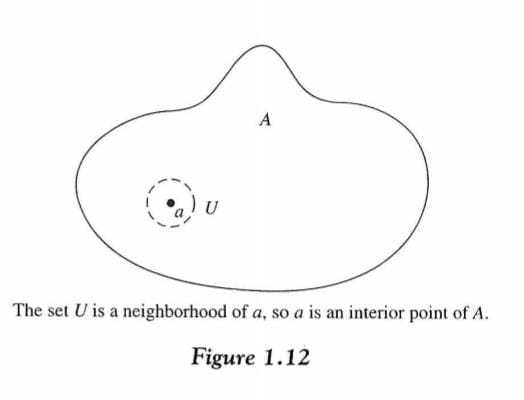
\includegraphics[width=3cm]{pembagian/Figure 1.12.jpg}
        \label{fig:enter-label}
    \end{figure}

    \end{tcolorbox}
Catatan:\\
Jika $A$ adalah subset dari ruang topologi ($\nX, \nT$) dan $B =$ \{$x \in \nX : x$ adalah titik interior dari $A$\}, maka $B =$ int($A$). Kemudian, jika ($\nX,d$) adalah ruang metrik, $A \subseteq \nX$ dan $x \in A $, maka $x$ $\in$ int($A$) jika dan hanya jika terdapat bilangan bulat positif $\epsilon$ sedemikian sehingga $B(x,\epsilon) \subseteq A$
\end{frame}

\begin{frame}{Teorema Interior}
    \begin{tcolorbox}[enhanced,title=Teorema 1.24, frame style tile={width=\paperwidth}{\wallpaper}]
        Misalkan $A$ dan $B$ adalah subset dari ruang topologi $(\nX, \nT)$, maka : 
        \begin{enumerate}
        \item $A$ buka jika dan hanya jika $A = int(A)$.
        \item Jika $A \subseteq B$ , maka $int(A) \subseteq int(B)$
        \item $int(A \cap B) = int($A$) \cap int(B)$
        \item $int(A) \cup int(B) \subseteq int(A \cup B)$
        \end{enumerate}
    \end{tcolorbox}
\end{frame}

\begin{frame}{Teorema Interior}
    \begin{tcolorbox}[enhanced,title=Teorema 1.24, frame style tile={width=\paperwidth}{\wallpaper}]
        1. Misalkan $A$ dan $B$ adalah subset dari ruang topologi ($\nX, \nT$), maka : \\
        $A$ buka jika dan hanya jika $A = int(A)$. \\

        Bukti : [Lihat Exercise 10]
        
    \end{tcolorbox}
\end{frame}

\begin{frame}{Teorema Interior}
    \begin{tcolorbox}[enhanced,title=Teorema 1.24, frame style tile={width=\paperwidth}{\wallpaper}]
        Misalkan $A$ dan $B$ adalah subset dari ruang topologi ($\nX, \nT$), maka : \\
        2. Jika $A \subseteq B$ , maka $int(A) \subseteq int(B)$ \\
        Bukti :
        \begin{itemize}
            \item Misalkan $A \subseteq B$, akan dibuktikan jika $x \in int(A)$ maka $x \in int (B)$
            \item Ambil sembarang $x \in int(A)$.
            \item Karena $x \in int(A)$, maka berdasarkan definisi, terdapat lingkungan U dari x sehingga $U \subseteq A$
            \item karena $U \subseteq A $ dan $A \subseteq B$, maka $U \subseteq B$ sehingga $x \in int (B)$
            \item Karena $x \in int (B)$, maka $int(A) \subseteq int(B)$
        \end{itemize}
    \end{tcolorbox}
\end{frame}

\begin{frame}{Teorema Interior}
    \begin{tcolorbox}[enhanced,title=Teorema 1.24, frame style tile={width=\paperwidth}{\wallpaper}]
        Misalkan $A$ dan $B$ adalah subset dari ruang topologi ($\nX, \nT$), maka : \\
        3. $int(A \cap B) = int(A) \cap int(B)$ \\

        Bukti : [Lihat Exercise 10]
        
    \end{tcolorbox}
\end{frame}

\begin{frame}{Teorema Interior}
    \begin{tcolorbox}[enhanced,title=Teorema 1.24, frame style tile={width=\paperwidth}{\wallpaper}]
        Misalkan $A$ dan $B$ adalah subset dari ruang topologi ($\nX, \nT$), maka : \\
        4. $int(A) \cup int(B) \subseteq int(A \cup B)$
    \end{tcolorbox}
\end{frame}

\begin{frame}{Teorema Interior}
    \begin{tcolorbox}[enhanced,title=Teorema 1.24, frame style tile={width=\paperwidth}{\wallpaper}]
        Bukti :
        \begin{itemize}
            \item Ambil sembarang $x \in int(A) \cup int(B)$. Akan dibuktikan $x \in int(A \cup B)$
            \item karena $x \in int(A) \cup int(B)$ maka $x \in int(A)$ atau $x \in int(B)$
            \item Karena $x \in int(A)$ maka berdasarkan definisi, terdapat lingkungan $U$ dari $x$ sehingga $U \subseteq A$
            \item Karena $x \in int(B)$ maka berdasarkan definisi, terdapat lingkungan $U$ dari $x$ sehingga $U \subseteq B$
            \item Pada kedua kasus, maka $U \subseteq A \cup B$, sehingga $x \in int(A \cup B)$ 
            \item Karena $x \in int(A \cup B)$ maka $int(A) \cup int(B) \subseteq int(A \cup B)$
        \end{itemize}
        
    \end{tcolorbox}
\end{frame}

\begin{frame}{Contoh 48}
    \begin{tcolorbox}[enhanced,title= Contoh 48, frame style tile={width=\paperwidth}{\wallpaper}]
        Misalkan $\nF$ adalah usual topologi di $\R$, misalkan juga $A$ = [$0, 1$] dan $B$ = [$1, 2$], Maka int($A \cup B$) = ($0,2$). Namun, int($A$) = ($0,1$) dan int($B$) = ($1,2$) sehingga $int($A$) \cup int(B) = (0,1) \cup (1,2)$

        
    \end{tcolorbox}
\end{frame}

\begin{frame}{Nowhere Dense}
    \begin{tcolorbox}[enhanced,title= Definisi, frame style tile={width=\paperwidth}{\wallpaper}]
        Suatu subset $A$ dari ruang topologi dikatakan \textbf{nowhere dense} jika memenuhi $int(\bar{A}) = \varnothing$
    \end{tcolorbox}
\end{frame}

\begin{frame}{Relative Discrete}
    \begin{tcolorbox}[enhanced,title= Definisi, frame style tile={width=\paperwidth}{\wallpaper}]
        Suatu subset $A$ dari ruang topologi ($\nX, \nT$) dikatakan \textbf{relatively discrete} jika untuk setiap $a \in A$, terdapat $U \in \nT$ sedemikian sehingga $U \cap A$ = \{$a$\}
    \end{tcolorbox}
\end{frame}

\begin{frame}{Teorema 1.25}
    \begin{tcolorbox}[enhanced,title= Teorema 1.25, frame style tile={width=\paperwidth}{\wallpaper}]
        Misalkan ($\nX, \nT$) adalah ruang topologi, Misalkan $C$ merupakan subset tutup dari $\nX$ dan misalkan $U$ adalah subset buka dari $\nX$, maka $C - U$ tutup dan $U - C$ Buka. \\
        Bukti : [Lihat Exercise 29]
    \end{tcolorbox}
\end{frame}

\begin{frame}{Teorema 1.26}
    \begin{tcolorbox}[enhanced,title= Teorema 1.26, frame style tile={width=\paperwidth}{\wallpaper}]
        Misalkan ($\nX, d$) adalah ruang metrik, Misalkan $x \in \nX$ dan misalkan $\epsilon$ dan $\delta$ adalah bilangan bulat positif yang memenuhi $\delta < \epsilon$, maka $\overline{B(x,\delta)} \subseteq B(x,\epsilon)$  \\
        Bukti : [Lihat Exercise 30]
    \end{tcolorbox}
\end{frame}

\begin{frame}{Perfect Set}
    \begin{tcolorbox}[enhanced,title= Definisi, frame style tile={width=\paperwidth}{\wallpaper}]
        Suatu Subset $A$ dari ruang topologi ($\nX, \nT$) dikatakan \textbf{perfect set} jika $A$ = $A'$  \\
    \end{tcolorbox}
\end{frame}

\begin{frame}{Isolated Point}
    \begin{tcolorbox}[enhanced,title= Definisi, frame style tile={width=\paperwidth}{\wallpaper}]
        Suatu titik $x$ dari subset A dari ruang topologi ($\nX, \nF$) dikatakan \textbf{isolated point} jika terdapat lingkungan $x$ yang tidak memuat titik $A$ yang berbeda dari $x$.

    \end{tcolorbox}
\end{frame}

\begin{frame}{Perfect Set}
    \begin{tcolorbox}[enhanced,title= Teorema 1.27, frame style tile={width=\paperwidth}{\wallpaper}]
        Suatu subset $A$ dari ruang topologi ($\nX, \nF$) dikatakan \textbf{perfect set} jika dan hanya jika subset tersebut tutup dan tidak punya \textbf{isolated point} \\
        Bukti : [Lihat Exercise 24]

    \end{tcolorbox}
\end{frame}

\end{document}